\chapter{Lateral Control}

\section{Exercise 1 - lateral control}
\textbf{Q. Optimize the clothoid-based lateral controller}

The clothoid-based lateral controller uses Equation \ref{eq:6.1} to calculate the steering angle required to follow the clothid. The under-steering gradient $\kus$ was calculated previously using the handling diagram shown in Table \ref{tab:5.1}. These results were implemented as a variable that changes based on the vehicle's current speed.

\begin{equation}\label{eq:6.1}
\delta(s) = k(s) (L + \kus u^2)
\end{equation}

To optimize the clothoid-based lateral controller look ahead variable, several tests were conducted using the following variables totalling 42 tests:

\begin{itemize}
    \item $u$ = [10, 20, 30, 40, 50, 60, 70, 80] km/h
    \item look ahead = [5, 10, 15, 20, 25, 30]
\end{itemize}

The tracking error had to be calculated to compare the tests' results. That was done by using the ``N-D nearest point search" function in Matlab, which returns indices of closest points in the desired path for each point on the real path. Then calculating the euclidean distance between each point in the real path and closest point on the desired path as tracking error. The results are shown in Figure \ref{61a-4} and Table \ref{tab:6.1} where LA is the look ahead value.
        
        \begin{figure}[ht]
        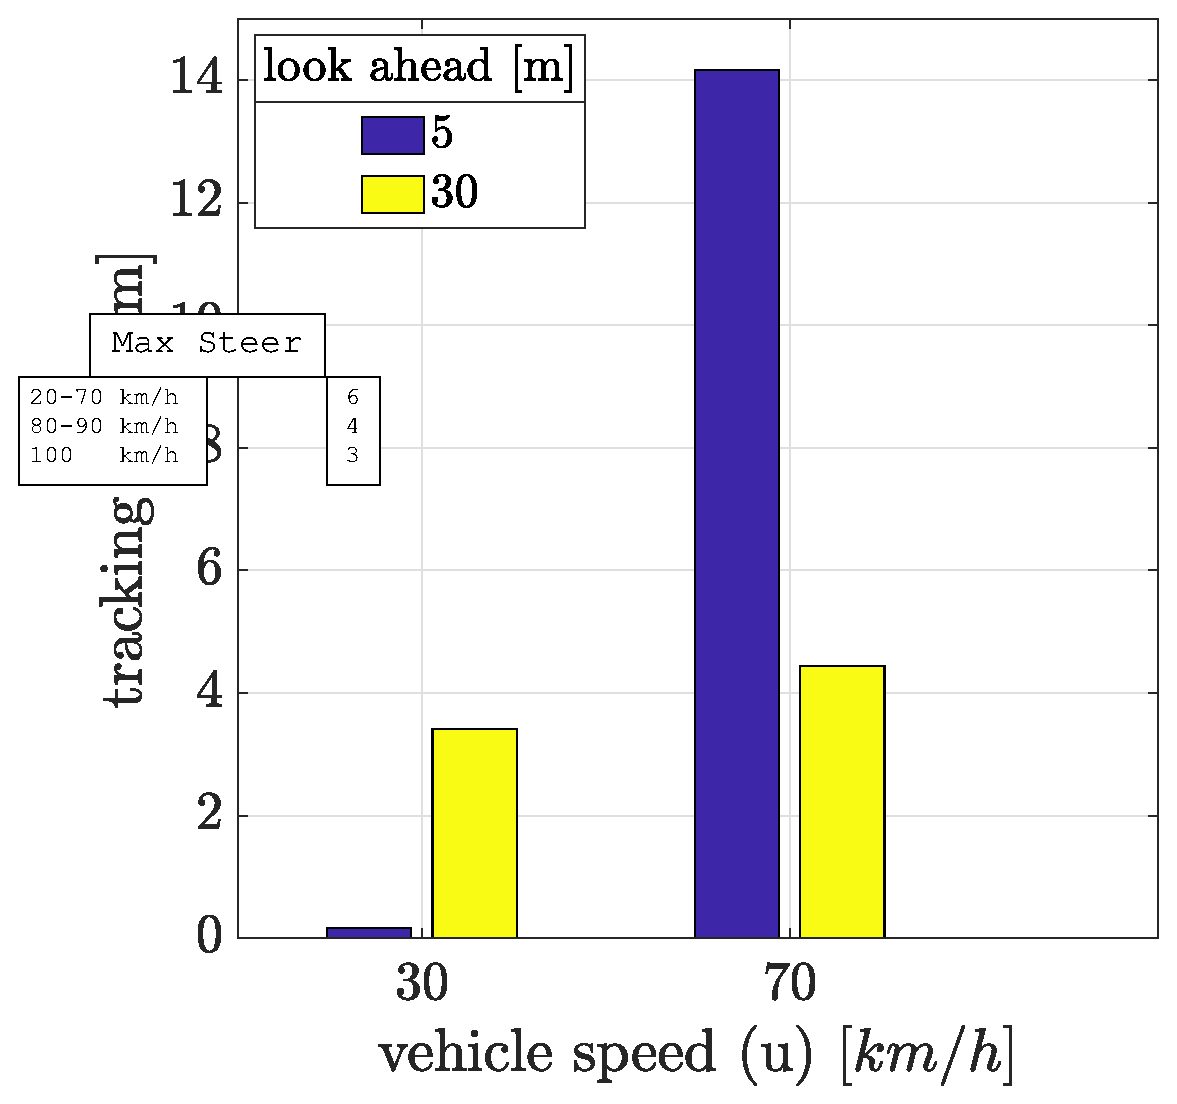
\includegraphics[width=0.6\linewidth]{ex6/q1/ex-61a-4.eps}
        \centering
        \caption{clothoid-based lateral controller at different $u$ and look ahead}
        \label{61a-4}
        \end{figure}
      
The tests checked if the vehicle was able to arrive at a designated target point chosen to be at [60,10]. If the vehicle reaches this point within a threshold of 5 meters, the test is considered a success.

\begin{table}[ht]
    \centering
    \begin{tabular}{c | c | c| c | c | c | c }
      \textbf{$u$ [km/h]} & \textbf{LA = 5} & \textbf{LA = 10} & \textbf{LA = 15} & \textbf{LA = 20} & \textbf{LA = 25} & \textbf{LA = 30} \\ \hline
      20 &  \cellcolor{green!10}\num{0.212718999}	& \num{0.481794113}	& \num{1.025936442} &	\num{1.72651936}	& \num{2.534489657}	& \num{3.45986332}   \\\hline
      30 &  \cellcolor{green!10}\num{0.163715271} &	\num{0.431919243} &	\num{0.941254925} &	\num{1.632800857} &	\num{2.454559877} &	\num{3.408670041}\\\hline
      40 &  \cellcolor{green!10}\num{0.225603124} & \num{0.361992743}	& \num{0.728903508} &	\num{1.387858567} &	\num{2.228111216} &	\num{3.252073013}  \\\hline
      50 & \cellcolor{red!10}NA & \num{9.077008353} & \num{1.421928047} & \cellcolor{green!10}\num{0.718803621} &	\num{1.593478851} & \num{2.81030173} \\\hline
      60 &  \cellcolor{red!10}NA & \num{12.14781879} &	\num{8.667722795}	& \cellcolor{green!10}\num{3.2567} & \num{5.819637} & \num{9.074008} \\\hline
      70 &  \num{14.15735028} & \num{23.03289356} & \cellcolor{red!10}NA & \cellcolor{red!10}NA & \num{4.14466} & \cellcolor{green!10}\num{4.4459637}

    \end{tabular}
    \caption{Tracking error results [clothoid-based lateral controller]}
    \label{tab:6.1}
\end{table}

The red colored cells indicates the vehicle was not able to arrive at the designated target point. Green cells are the chosen look ahead values at each speed $u$.

It appears that the larger the look ahead value, the larger the tracking error as expected. Having a larger look ahead at 20 km/h could be beneficial if we are optimizing for traveled distance, and smoother turns [less jerk].

Figure \ref{61x20} shows the vehicle actual path at each look ahead value for 20 km/h tests. A larger look ahead optimized the vehicles path to take a shorter route and take better turns. However, this caused the tracking error to increase, because we are not following the reference trajectory anymore.

       \begin{figure}[ht]
        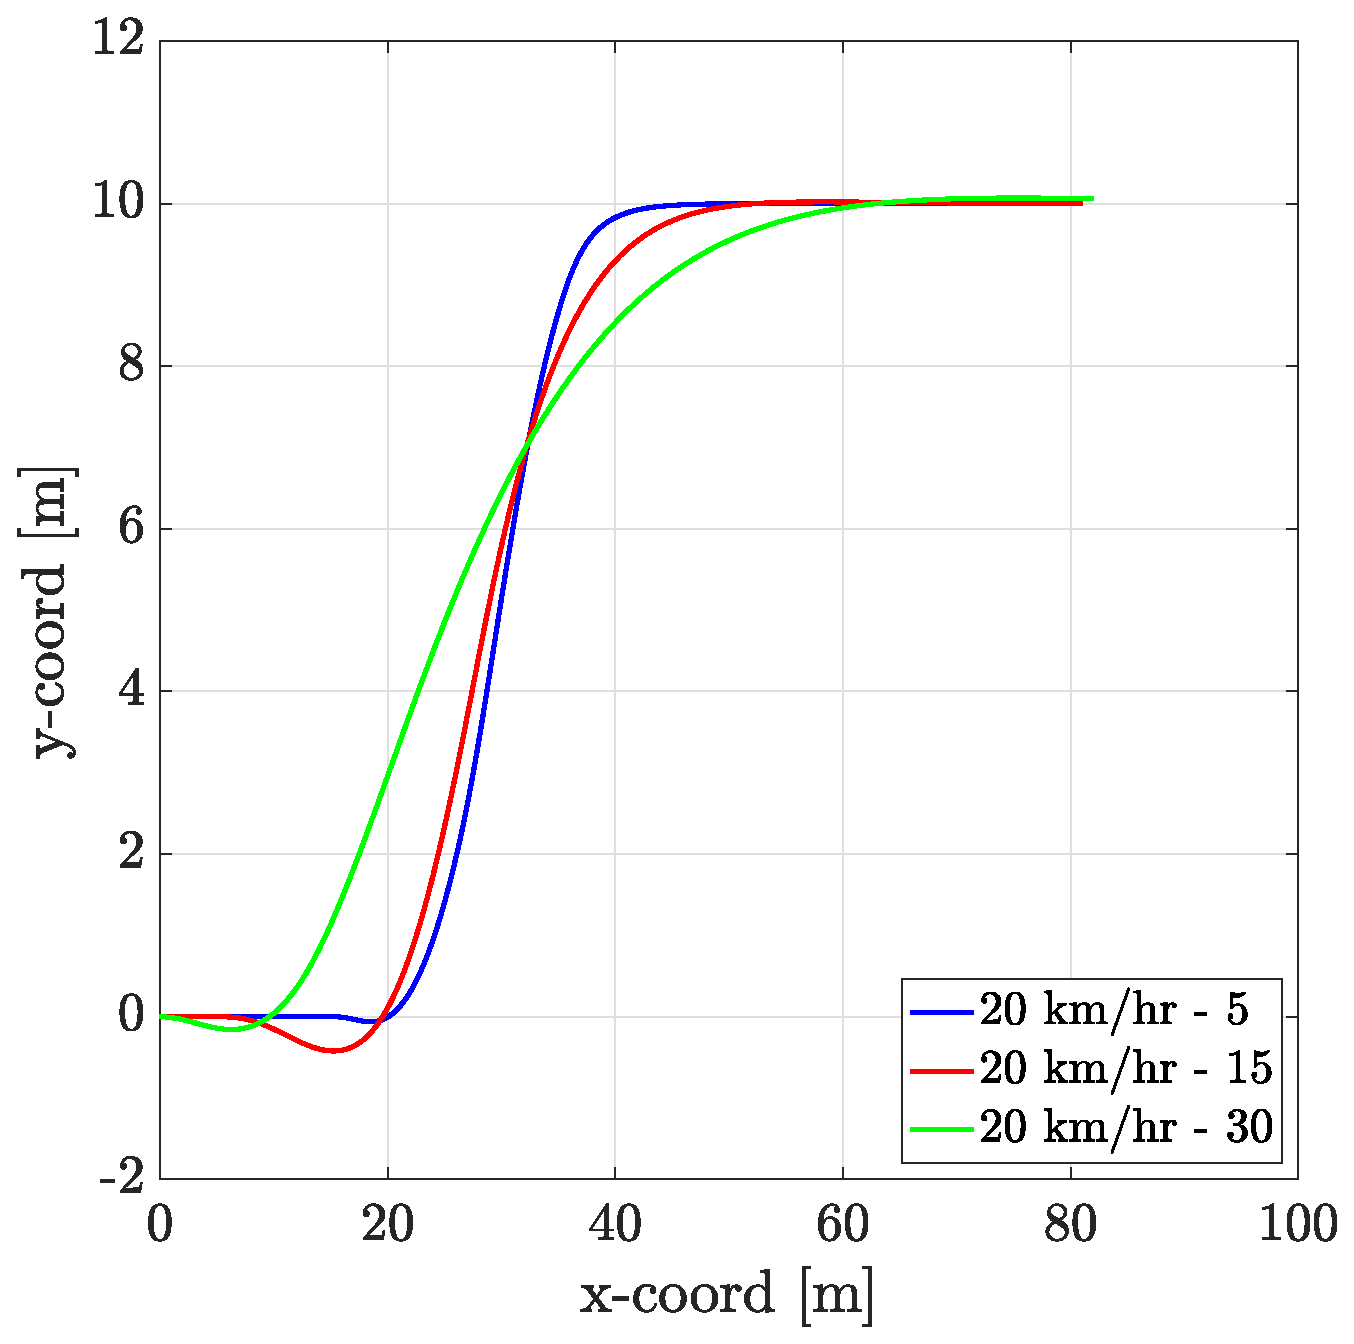
\includegraphics[width=0.6\linewidth]{ex6/q1/ex-61x20.eps}
        \centering
        \caption{Real vehicle path with different look ahead values [$u$ = 20km/h] }
        \label{61x20}
        \end{figure}

Up until 40 km/h, a lower look ahead value performed better for our metrics. With increasing $u$, the smaller look ahead values were simply not enough to control the vehicle properly. The controller needs to see far enough ahead to account for a curve earlier on. The faster the vehicle, the bigger the needed look ahead value. However, it seems that after 70 km/h, the vehicle can no longer become stable even with a look ahead as high as 250. 

Figure \ref{61x70} shows the vehicle paths at 70 km/h at different values for the look ahead. The higher values are more stable but still considered outside the capabilities of the vehicle.

No values of look ahead was enough to stabilize the vehicle with any speed higher than 70 km/h. This might be attributed to the $\kus$ values not being accurate enough at these speeds. The handling curves during these speeds were not linear anymore and a linear approximation for them is not sufficient.

        \begin{figure}[ht]
        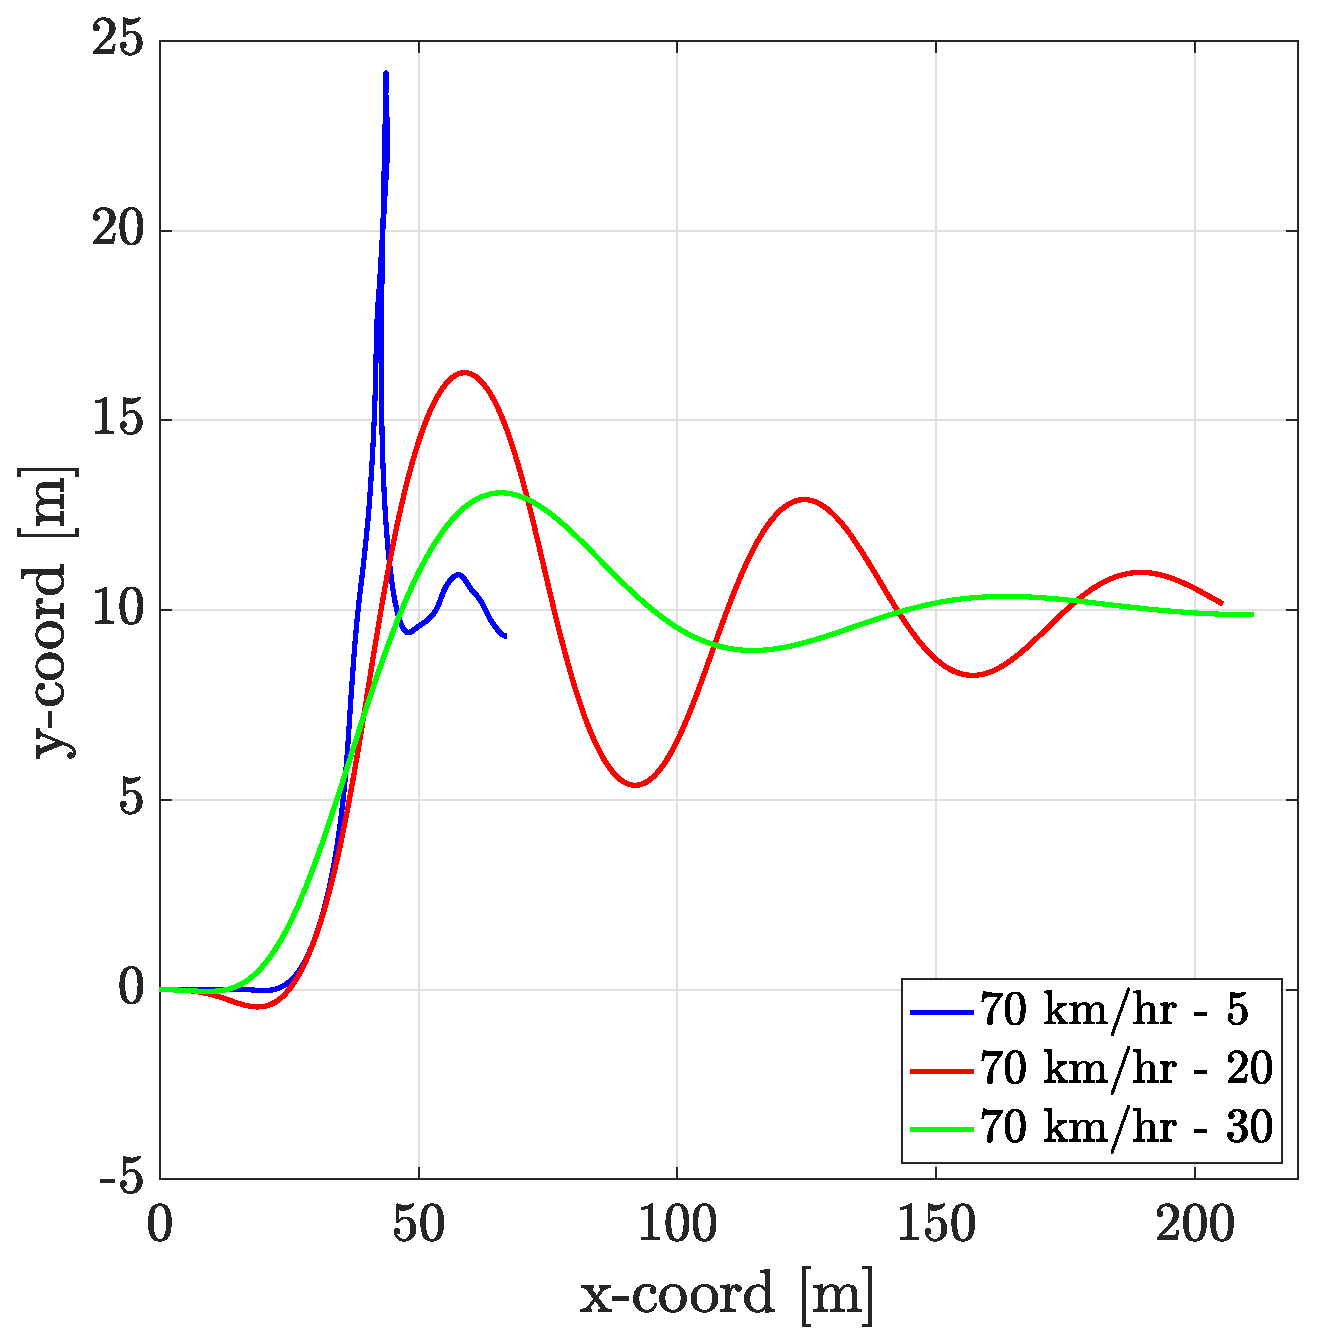
\includegraphics[width=0.6\linewidth]{ex6/q1/ex-61x70.eps}
        \centering
        \caption{Real vehicle path with different look ahead values[$u$ = 70km/h] }
        \label{61x70}
        \end{figure}

\textbf{Q. Implement the pure pursuit controller and optimize the look ahead distance}      

Pure pursuit calculates the circular arc radius $R$ between center of the vehicle's rear wheel $P_{V}$ and the target point on the desired path $P_{D}$. Equation \ref{eq:6.2} is used to calculate $R$, where $x_{D} $ and $y_{D}$ are $P_{D}$ expressed in the vehicle's frame. $R$ is later used to calculate the required steering angle $\delta$.

\begin{equation}\label{eq:6.2}
R = \frac{\sqrt{x_{D}^2 + y_{D}^2}}{2 sin(\lambda)} \quad\mathrm{and}\quad \delta = arctan(L/R)
\end{equation}

To optimize the pure pursuit lateral controller look ahead variable, several tests were conducted using the following variables totalling 64 tests:

\begin{itemize}
    \item $u$ = [20, 30, 40, 50, 60, 70, 80, 90, 100] km/h
    \item look ahead = [1, 2, 3, 4, 5, 10, 15, 20, 25, 30]
\end{itemize}

The tracking error was calculated in the same manner as previous and some of the results are shown in Figure \ref{62a-1} and Table \ref{tab:6.2}. The effect of the look ahead variable on the pure pursuit controller behaviour is similar to the clothoid-based controller. With higher speeds, larger look ahead values are required.
        \begin{figure}[ht]
        \includegraphics[width=0.6\linewidth]{ex6/q2/ex-62a-1.eps}
        \centering
        \caption{pure pursuit lateral controller at different $u$ and look ahead}
        \label{62a-1}
        \end{figure}

Overall, the pure pursuit controller performed well. Table \ref{tab:6.2} shows some of the tests conducted and their tracking error. The red colored cells indicate the vehicle was not able to arrive at the target point, while the green cells are the best performers for each speed $u$. A look-up table can now be used to choose the correct look ahead based on current speed.

\begin{table}[ht!]
    \centering
    \begin{tabular}{c | c | c| c | c | c | c }
      \textbf{$u$ [km/h]} & \textbf{LA = 3} & \textbf{LA = 10} & \textbf{LA = 15} & \textbf{LA = 20} & \textbf{LA = 25} & \textbf{LA = 30} \\ \hline
      20 &  \cellcolor{green!10}\num{0.122447479884261}	& \num{1.20229858149544}	& \num{1.98665627365860} &	\num{2.50901222735532}	& \num{2.89607564298269}	& \num{3.36310387417133}   \\\hline
      40 &  \cellcolor{green!10}\num{0.545850027367760} &	\num{0.903114425955597} &	\num{1.73093343366169} &	\num{2.31062509178793} &	\num{2.73594362776234} &	\num{3.23567396181456}\\\hline
      60 &  \num{14.9833184394890} & \num{14.9378800339917}	& \num{11.62915169313966} &\cellcolor{green!10}	\num{2.05379295557061} &	\num{2.47442576799508} &	\num{3.02057477231781}  \\\hline
      80 & \cellcolor{red!10}NA & \cellcolor{red!10}NA & \cellcolor{red!10}NA & \cellcolor{green!10}\num{2.76118476320162} &	\num{2.61057892579461} & \num{3.06265625323397} \\\hline
      100 &  \cellcolor{red!10}NA & \cellcolor{red!10}NA &	\cellcolor{red!10}NA & \cellcolor{red!10}NA  & \cellcolor{red!10}NA  & \cellcolor{green!10}\num{3.78184237059937}

    \end{tabular}
    \caption{Tracking error results [pure pursuit lateral controller]}
    \label{tab:6.2}
\end{table}

\textbf{Q. Evaluate the performance of the Stanley kinematic and dynamic controllers}

The Stanley kinematic controller is mainly suitable for low speeds because it does not make use of a look ahead parameter. The absolute value of the path tracking error is the distance between the center of the vehicle's front wheel $P_{F}$ and the closest point of the path $P_{P}$  w.r.t $P_{F}$.

\begin{equation}\label{eq:6.3}
\lvert e\rvert = \overline{P_{F}P_{P}} \quad\mathrm{and}\quad \delta = \delta \theta + arctan(\frac{\ke . e}{\vf})
\end{equation}

To evaluate the Stanley kinematic controller, several tests were conducted using the following variables totalling 27 tests. The results are shown in Figure \ref{63a-2} and Table \ref{tab:6.3}:

\begin{itemize}
    \item $u$ = [20, 30, 40, 50, 60, 70, 80, 90, 100] km/h
    \item Gain $\ke$ = [0.1, 0.5, 1]
\end{itemize}

        \begin{figure}[ht]
        \includegraphics[width=0.63\linewidth]{ex6/q3/ex-63a-2.eps}
        \centering
        \caption{Stanley kinematic lateral controller at different $u$ and gain $\ke$}
        \label{63a-2}
        \end{figure}


\begin{table}[ht]
    \centering
    \begin{tabular}{c | c| c| c}
      \textbf{$u$ [km/h]}  & \textbf{$\ke$ = 0.1} & \textbf{$\ke$ = 0.5} & \textbf{$\ke$ = 1}\\ \hline
      20 &  \num{0.542409430254252} &  \num{0.508090176246383}  &  \cellcolor{green!10}\num{0.487699025938634}     \\\hline
      40 &  \cellcolor{green!10}\num{1.69518298558262} &  \num{1.84728050038547}  &  \num{2.63907755509404}  \\\hline
      60 &  \cellcolor{green!10}\num{4.78256353896437} &  \num{5.94323455084316} &  \num{7.22202999952100} \\\hline
      80 &  \cellcolor{green!10}\num{6.28022019561736} &  \cellcolor{red!10}NA &  \cellcolor{red!10}NA \\\hline
      100 &  \cellcolor{green!10}\num{8.34514063115690} &  \num{8.34453282013186} &  \num{8.34397987275621} \\
    \end{tabular}
    \caption{Tracking error results [Stanley kinematic lateral controller]}
    \label{tab:6.3}
\end{table}

It is important to note that the max steering angle had to be changed for the higher speeds in order for the controller to stabilize the vehicle [shown on Figure \ref{63a-2}]. As expected, the Stanley kinematic lateral controller works well with lower speeds, and struggles with speeds higher than 60 km/hr for our vehicle.

The Stanley dynamic controller uses a similar equation as the kinematic controller to calculate $\delta$, except it has an extra gain parameter $\ky$ to actively dampen the yaw rate dynamics during high speeds.

\begin{equation}\label{eq:6.4}
\delta = \delta \theta + arctan(\frac{\ke . e}{\vf}) + \ky (\Omega_{t} - \Omega)
\end{equation}

The evaluation for the Stanley dynamic lateral controller followed the same test process as the kinematic one. Both gains $\ke$ and $\ky$ were changed simultaneously with the same value for each test. The results are shown in Figure \ref{63a-3} and Table \ref{tab:6.4}.

Similar to the kinematic controller, the dynamic controller needed smaller maximum steering angles with higher speeds to stabilize the vehicle [shown on Figure \ref{63a-3}]. However, the overall performance of the dynamic controller was better than the kinematic version.

        \begin{figure}[ht]
        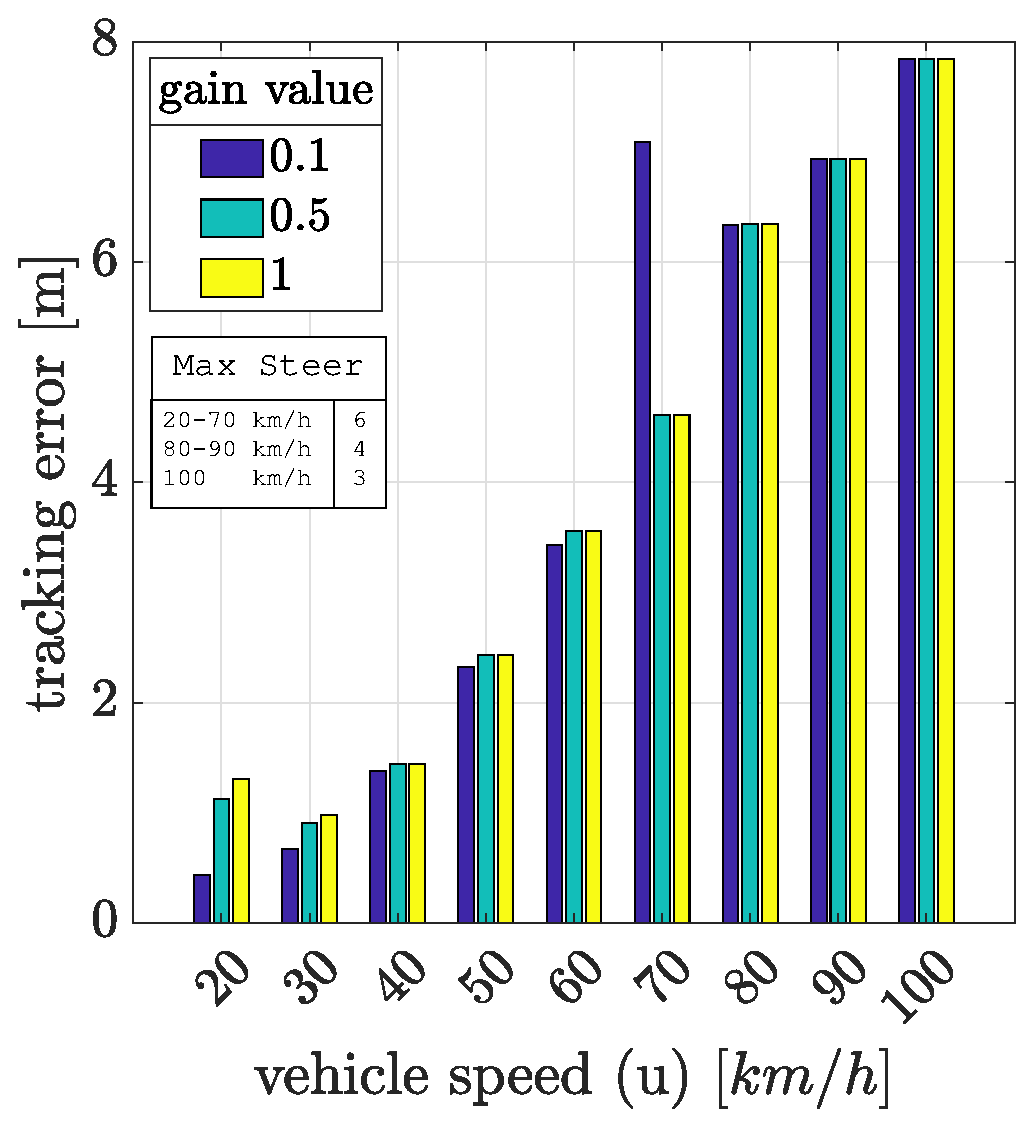
\includegraphics[width=0.5\linewidth]{ex6/q3/ex-63a-3.eps}
        \centering
        \caption{Stanley dynamic lateral controller at different $u$ and gain $\ke$ and $\ky$}
        \label{63a-3}
        \end{figure}


\begin{table}[ht]
    \centering
    \begin{tabular}{c | c| c| c}
      \textbf{$u$ [km/h]}  & \textbf{$\ke$/$\ky$ = 0.1} & \textbf{$\ke$/$\ky$ = 0.5} & \textbf{$\ke$/$\ky$ = 1}\\ \hline
      20 &  \cellcolor{green!10}\num{0.433870147950401} &  \num{1.12319636881579}  &  \num{1.30816540263685}     \\\hline
      40 &  \cellcolor{green!10}\num{1.37630980207272} &  \num{1.43951495823005}  &  \num{1.44215501293828}  \\\hline
      60 &  \cellcolor{green!10}\num{3.43271937243360} &  \num{3.55734662611000} &  \num{3.55734662611000} \\\hline
      80 &  \cellcolor{green!10}\num{6.33232256752558} &  \num{6.34432776705650} &  \num{6.34432776705650} \\\hline
      100 &  \cellcolor{green!10}\num{7.84331899204944} &  \num{7.84331899204944} &  \num{7.84331899204944} \\
    \end{tabular}
    \caption{Tracking error results [Stanley dynamic lateral controller]}
    \label{tab:6.4}
\end{table}


\textbf{Q. Compare the performance of the lateral controllers}


        \begin{figure}[ht!]
        \includegraphics[width=0.5\linewidth]{ex6/q4/ex-64er.eps}
        \centering
        \caption{Lateral controllers maximum tracking error comparison at different $u$}
        \label{64er}
        \end{figure}
   
   
The comparison will be based on the maximum tracking error and the steering behaviour. One example of a low speed (30 km/h) and high speed (70 km/h) run was chosen for each controller. The best performing hyper parameters [look ahead, gains, max steer angle] for each controller were chosen based on the tests previously conducted. The tracking error results are shown in Figure \ref{64er}.

From a tracking error metric prospective, the pure pursuit controller performed the best on both low and high speeds. It was capable of maintaining stability at much higher speeds. As a comparison, pure pursuit was able to achieve target up to 130 km/hr, while the other controllers had trouble with any speed over 70 km/hr. Furthermore, pure pursuit requires only one hyper-parameter to tune.

On the other side of the spectrum, Stanley Kinematic was the worst performer on both low and high speeds. For both the Stanely controllers, it was no surprise they would not perform well, especially on higher speeds due to the lack of a look ahead feature. 

        \begin{figure}[ht]
        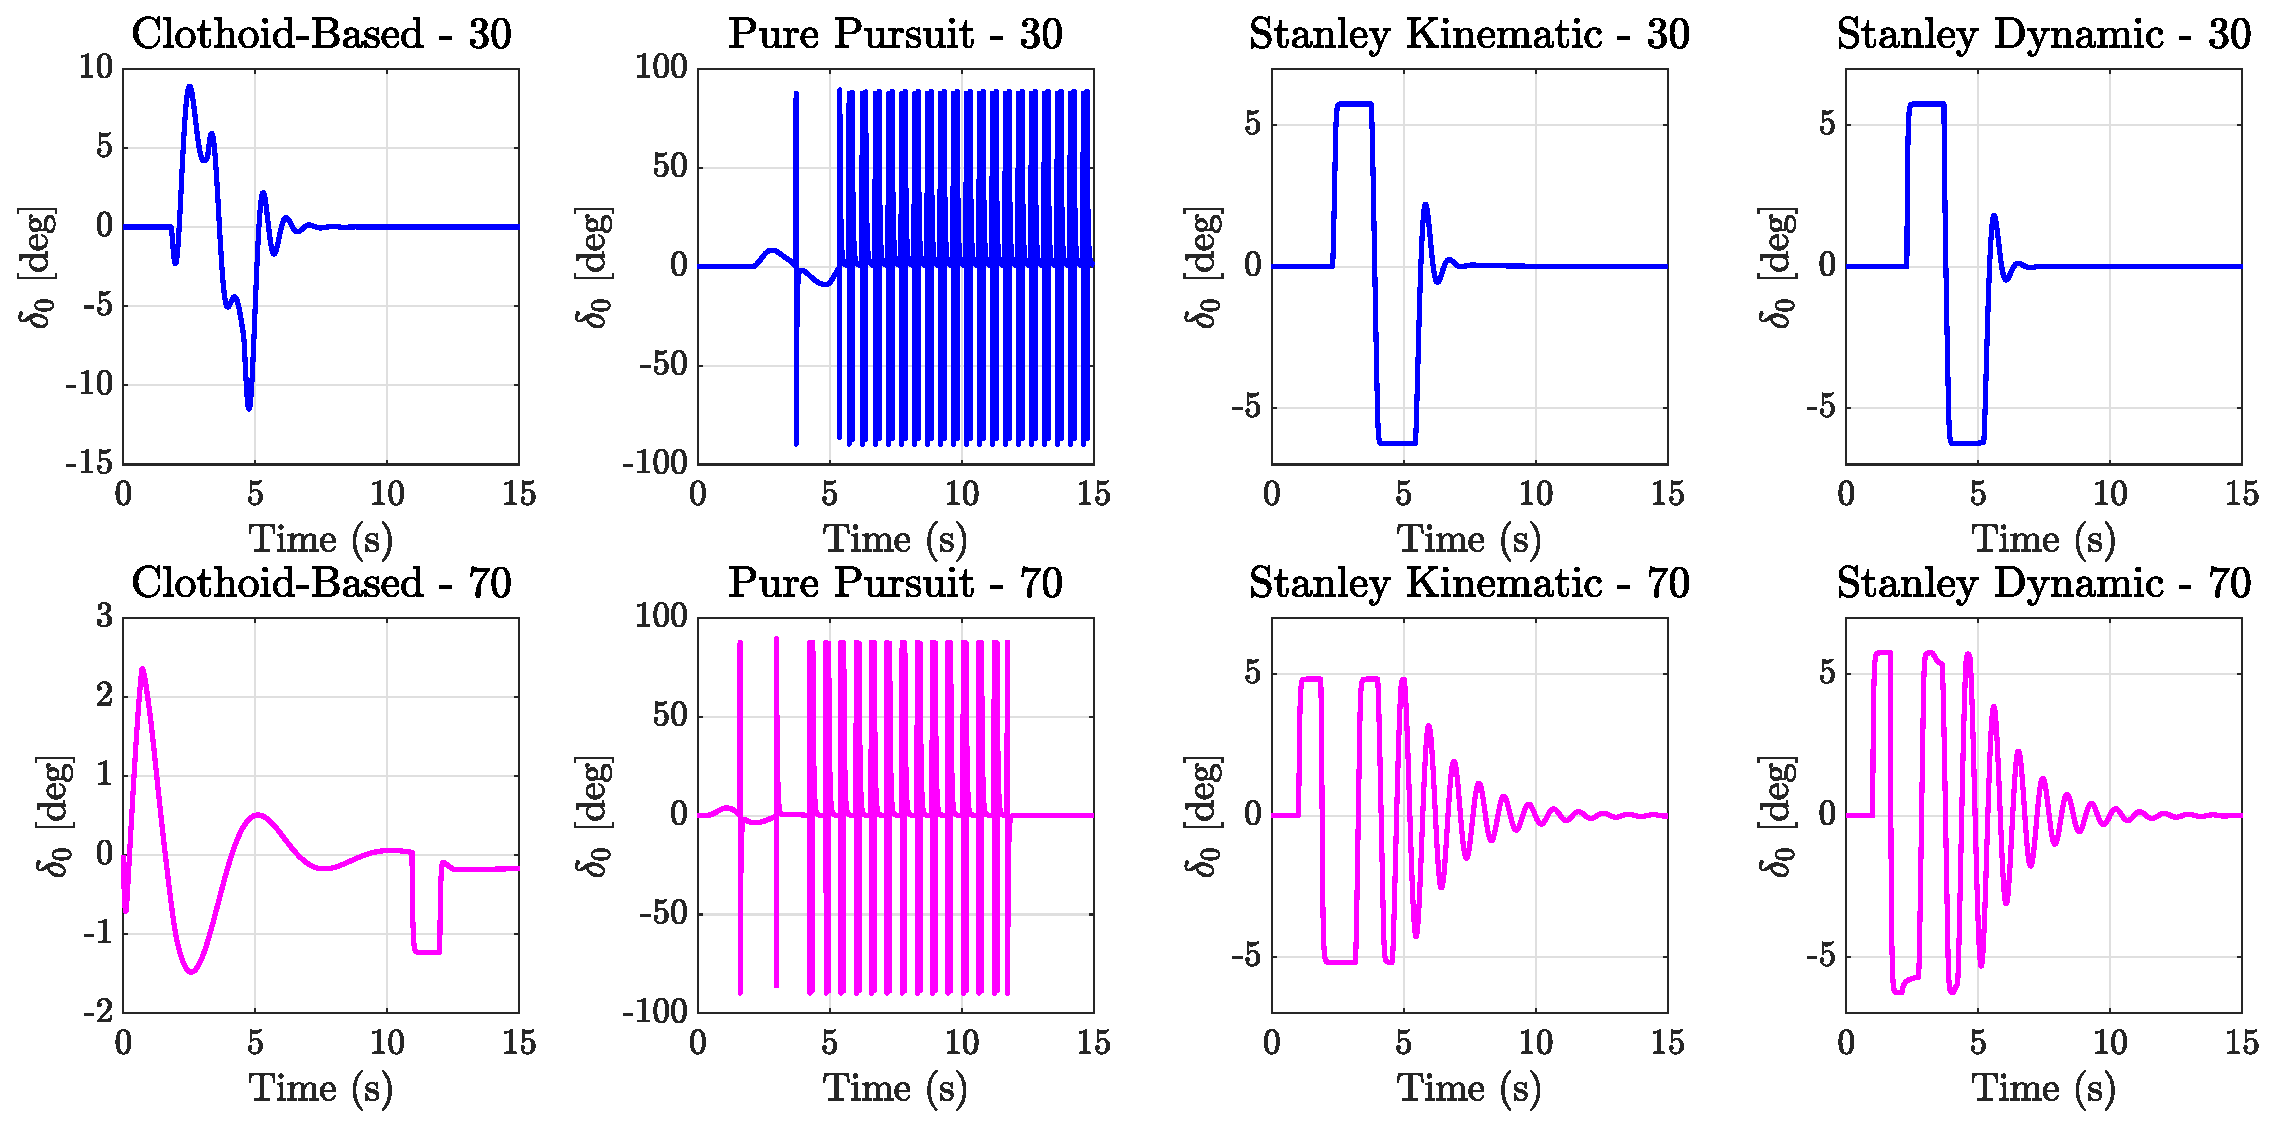
\includegraphics[width=0.99\linewidth]{ex6/q4/ex-64ff.eps}
        \centering
        \caption{Lateral controllers steering behaviour comparison at different $u$}
        \label{64ff}
        \end{figure}
        
The steering angles for the same chosen runs are plotted in Figure \ref{64ff}. The steering angle for pure pursuit exhibited the best smoothness in steering with no sudden jerky changes. It would be a pleasant ride in a vehicle using this controller.   
        
The clothoid based controller is trailing slightly behind pure pursuit as it showed more sudden transitions between angles, which could make it a less comfortable ride compared to the pure pursuit.

Both of the Stanley controllers showed the same pattern. Some oscillation were present at the higher speed run.

Overall, from a tracking error prospective, and steering behaviour, the pure pursuit lateral controller is a clear winner compared to the rest of the controllers tested.

\textbf{Q. Underline the pros and cons of each algorithm}
\begin{table}[ht!]
    \centering
    \begin{tabular}{m{0.14\linewidth}|m{0.39\linewidth}|m{0.39\linewidth}} 
       \textbf{Controller} & \textbf{Pros} & \textbf{Cons} \\
        \hline
        
         Clothoid-based & 
        
    % \begin{minipage}[t]{\linewidth}
    \setlist{leftmargin=*}
    \begin{itemize}[noitemsep]
        \item smooth steering behaviour
        \item benefits from knowledge of the vehicle's handling behaviour
        \item best overall performer at lower speeds
    \end{itemize}
    % \end{minipage} 
    &

    % \begin{minipage}[t]{\linewidth}
    \setlist{leftmargin=*}
    \begin{itemize}[noitemsep]
        \item requires 2 hyper parameters
        \item high computation cost
        \item poor on high speeds

    \end{itemize}
    % \end{minipage} 
    \\ \hline
        
        Pure pursuit & 
        
    % \begin{minipage}[t]{\linewidth}
    \setlist{leftmargin=*}
    \begin{itemize}[noitemsep]
        \item tracks reference very well
        \item simple to implement
        \item only 1 hyper parameter to tune
        \item low computation cost
        \item functions at very high speeds
    \end{itemize}
    % \end{minipage} 
    &

    % \begin{minipage}[t]{\linewidth}
    \setlist{leftmargin=*}
    \begin{itemize}[noitemsep]
        \item look ahead must be specific for each speed
        
    \end{itemize}
    % \end{minipage} 
    \\ \hline
        
        S. kinematic& 
        
    % \begin{minipage}[t]{\linewidth}
    \setlist{leftmargin=*}
    \begin{itemize}[noitemsep]
        \item low computation cost
        \item only 1 hyper parameter
        \item simple to implement
    \end{itemize}
    % \end{minipage}  
    & 

    % \begin{minipage}[t]{\linewidth}
    \setlist{leftmargin=*}
    \begin{itemize}[noitemsep]
        \item no look ahead feature
        \item doesn't do well in high speeds
    \end{itemize}
    % \end{minipage} 
    \\ \hline
        
        S. dynamic & 
        
    % \begin{minipage}[t]{\linewidth}
    \setlist{leftmargin=*}
    \begin{itemize}[noitemsep]
        \item works better on higher speeds than the kinematic version
        \item performs well on low speeds
    \end{itemize}
    % \end{minipage}
    & 

    % \begin{minipage}[t]{\linewidth}
    \setlist{leftmargin=*}
    \begin{itemize}[noitemsep]
        \item no look ahead feature
        \item requires 2 hyper parameters
        \item shows oscillations at higher speeds
    \end{itemize}
    % \end{minipage} 
    \\ 
    \end{tabular}
  \caption{Pros and Cons of lateral controllers}
  \label{tab:6.5}
\end{table}
